\chapter{Literature Review}
\label{ch:literature_review}

% =====================================================================
%   2.1 EoL problem .................  350   (1.0 pp)
%   2.2 TFC membranes ...............  650   (1.9 pp)
%   2.3 Ageing and fouling ..........  550   (1.6 pp)
%   2.4 Fouling vs regeneration ..... 1150   (3.3 pp)  <- protected
%   2.5 EoL management routes .......  450   (1.3 pp)
%   2.6 Polyamide regeneration ......  750   (2.1 pp)  <- protected
%   2.7 Research gaps ...............  250   (0.7 pp)
% =====================================================================

This chapter establishes why end-of-life (EoL) reverse osmosis (RO) membranes are worth recovering rather than discarding, then narrows to the two things that determine whether polyamide regeneration can work in practice: the condition of the polysulfone substrate it is built on, and the fouling layer that must be removed before a new film can form.
% Write LAST. Max 100 words.


% =====================================================================
\section{The end-of-life RO membrane problem}
\label{sec:eol-problem}

Reverse osmosis (RO) has emerged as the dominant desalination technology in desalination plants operational worldwide, and as of 2019, 15,906 desalination plants worldwide collectively produce around 95 million $\mathrm{m^3}$ of water per day \citep{Jones2019}. Despite attempts to improve service life, in most desalination applications, RO membranes typically remain in service for five to nine years \citep{Ding_2026, Lawler2015}. It is estimated that 5--20\% of membranes are replaced annually \citep{BerattoRamos2024, imdea2018transfomem, Guclu2022}, translating to a huge amount of polymeric waste. Increased global RO development and increasing water demands drives more membrane usage and waste. The lack of a viable recycling infrastructure makes EoL membranes a fast growing solid waste issue associated with water treatment.

Existing waste disposal techniques employed for EoL membranes currently mainly include landfill and incineration \citep{Khanzada2024}. Because the module is almost entirely polymeric (polyester, polysulfone, polyamide and polypropylene), it is classified as an intert municipal solid waste and the material only degrades approximately 1--5\% over 100 years \citep{Lawler2015}. In land-constrained countries such as Japan and Singapore, incineration is used instead \citep{Lawler2015}. Incineration reduces the waste volume and partly recovers the thermal energy, but the combustion of the polymers can release a range of harmful gasses including NO$_x$ and SO$_2$. Incineration produces a higher CO$_2$-equivalent emission than any reuse or recycling route \citep{Lawler2015}.

Both routes discard the element completely while it still holds recoverable value. An EoL membrane element maintains most of its PET and polysulfone support structural integrity \citep{Molinaa2018}. Directly reusing an EoL membrane offsets around 33\% of the environmental impact of manufacturing a replacement \citep{Lawler2015}. The alternative to disposal do not recover the value of a working RO membrane and permanently removes the high selectivity. This chapter aims to question whether the functionality of EoL RO membranes can be restored by replacing the polyamide layer on the recovered support, recovering the value of PET and PSF, while uplifting it's selectivity \citep{Ogbe2025,Ogbe2026}

% =====================================================================
\section{Thin-film composite RO membranes}
\label{sec:tfc-anatomy}
\flag{
Thin-film composite (TFC) RO membranes represent over 95\% of installed RO capacity globally \citep{Geise2010}. They comprise of three layers (Figure- \flag{Find TFC cross section})
\begin{itemize}
    \item \textbf{PET non-woven backing} (\textasciitilde120--150\,$\mu$m) \citep{LejarazuLarranaga2022}: provides tensile strength and withstands hydraulic pressure; the most porous, lowest resistance layer, and the largest mass fraction of the sheet \citep{Lawler2015}. It contributes to strength only.
    \item \textbf{Polysulfone (PSf) layer} (\textasciitilde40--150\,$\mu$m) \citep{LejarazuLarranaga2022}:  Supports the PA layer without adding excess hydraulic resistance \citep{Petersen1993} and is the surface of which PA is formed on.
    \item \textbf{Polyamide (PA) selective layer} (\textasciitilde0.2\,$\mu$m) \citep{LejarazuLarranaga2022}: Assembled via interfacial polymerisation of organic diamines and carboxylic acid monomers, typically using water as non-organic solvent and hexane as immiscible organic solvent. PA is responsible for the membrane's salt rejection and selectivity. 
\end{itemize}
}

\begin{figure}[htbp]
  \centering
  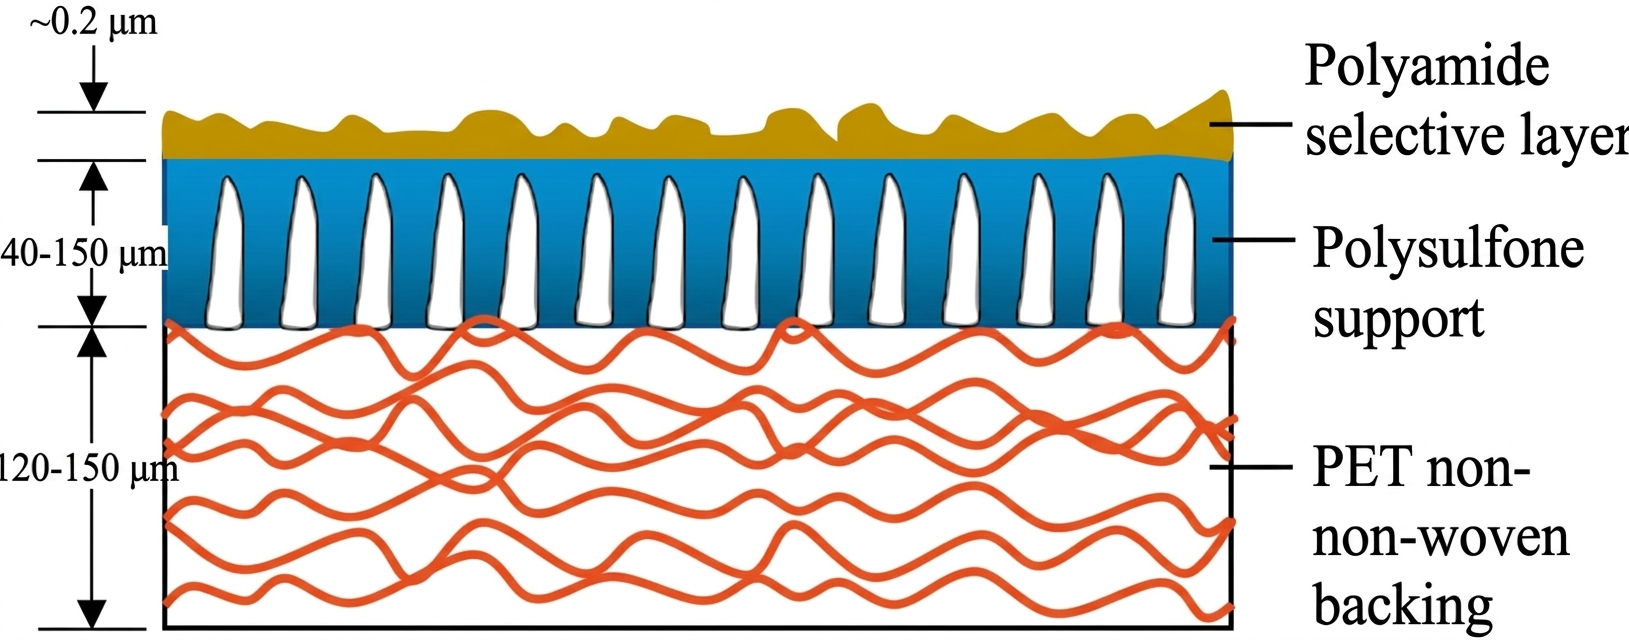
\includegraphics[width=0.8\textwidth]{figures/tfc_cross_section.jpg}
  \caption{Cross-section of a TFC RO membrane. Adapted from \citep{TFC_Composite_fig2020}}
  \label{fig:tfc-cross-section}
\end{figure}

Because the selectivity is largly concentrated at the PA layer and PA layer is the main site of chemical attack and fouling, regeneration aims to target the PA layer while preserving the PSf and PET beneath it. 


\subsection{Polyamide Formation by Interfacial Polymerisation}
\label{sec:lit-ip}

The PA layer is formed by interfacial polymerisation (IP) \citep{Petersen1993, Nunes2020}. An aqueous solution of m-phenylenediamine (MPD) is passed over the PSf support, then reacted with trimesoyl chloride (TMC), an immiscible organic solvent. The two monomers form a crosslinked aromatic PA network on the PSf surface \citep{Petersen1993}. As reaction time increase,

\begin{comment}
The PA layer is formed by interfacial polymerisation (IP)
\citep{Petersen1993, Nunes2020}. The PSf support is loaded with an
aqueous solution of m-phenylenediamine (MPD) and then contacted with
trimesoyl chloride (TMC) in an immiscible organic solvent; the two
monomers react where the phases meet, forming a crosslinked aromatic PA
network on the PSf surface \citep{Petersen1993}.
Film growth slows as the film builds: MPD diffuses rapidly across the
interface in the first 10--60\,s, but as the film thickens MPD
transport becomes restricted while TMC continues to diffuse, favouring
linear rather than crosslinked amide structure and yielding diminishing
rejection gains beyond about 60\,s \citep{Ogbe2026}.
 
The properties that determine separation performance are fixed at this
step. Film thickness and crosslink density govern the trade-off between
permeability and rejection \citep{Singh2006, PrakashRao2003}. Crosslink
density reflects the ratio of hydrolysed carboxylic acid groups to
crosslinked amide groups, and is sensitive to reaction time, humidity
and temperature \citep{PrakashRao2003}. Monomer concentration acts in the
same direction: raising MPD from 1.5 to 2.0\,wt\% increased NaCl rejection
from 96.8\% to 99.4\% but lowered pure water permeability from 6.3 to
1.4\,L\,m$^{-2}$\,h$^{-1}$\,bar$^{-1}$, with XPS O/N ratios falling from
1.21 to 1.09 across 1.0--2.0\,wt\% MPD, consistent with a denser network
\citep{Ogbe2026}.
\flag{CHECK - the old review called 6.3$\rightarrow$1.4 a ``40\% decline''.
It is a \textasciitilde78\% decline. Check the source figure.}
\flag{NEW - ridge-and-valley roughness, hydrophilicity and surface charge
as properties set during IP are not covered in the old review.}
 
What matters for the rest of this chapter is where the reaction takes
place. The MPD reservoir sits in the PSf, and the film forms at the PSf
surface \citep{Petersen1993, Singh2006}. Any change to that surface
therefore changes the film that forms on it.
\end{comment}

\subsection{The Polysulfone Substrate and Effect on Film Formation}
\label{sec:substrate}



% =====================================================================
\section{Ageing and fouling of RO membranes}
\label{sec:degradation}
% BUDGET: 550 words (~1.6 pp), split ~275 / 275.

\subsection{Chemical and mechanical degradation}
Covers oxidative attack and physical ageing together, distinguishing what regeneration can undo from what it cannot.


% ~275 words. Merged from three former subsections - keep it tight:
%   - N-chlorination, Orton rearrangement, amide hydrolysis; loss of
%     crosslinking -> rising permeability, falling rejection; ppm.h as
%     the controlling variable \citep{GarciaPacheco2015}
%   - compaction, delamination, support collapse: irreversible, and
%     therefore a ceiling on recoverable performance
%   - flag the duality once, briefly: the chemistry that destroys a
%     working membrane is the tool used to strip PA in Section 2.6.2
% The EoL performance signature (PWP, rejection, LRV, TMP) belongs in
% the Chapter 4 baseline table, NOT in prose here.

\subsection{Fouling classes and the fouling--cleaning cycle}
Identifies what accumulates on an RO membrane in service and why repeated cleaning accelerates its retirement.

% ~275 words. Compress the four foulant classes to roughly a sentence
% each - organic (humics, proteins, polysaccharides), inorganic scaling
% (CaCO3, CaSO4, silica), biofouling (cells + EPS), colloidal (clays,
% Fe/Al/Mn oxides). Note that real EoL elements carry composite,
% stratified, spatially heterogeneous fouling \citep{Molinaa2018}.
% Then the cycle: fouling raises TMP -> triggers cleaning -> cleaning
% damages PA -> damaged surface fouls faster.
% SIGNPOST: this subsection explains RETIREMENT; Section 2.4 addresses
% what the fouling layer does to REGENERATION.


% =====================================================================
\section{Fouling as a constraint on regeneration}
\label{sec:fouling-ip}
% BUDGET: 1,150 words (~3.3 pp) - the largest section in the chapter.
% Split ~300 / 400 / 250 / 200. This carries the novelty; protect it
% if the chapter needs further cutting elsewhere.
Establishes what survives cleaning and why residual foulants are expected to disrupt interfacial polymerisation, which is the central mechanistic argument of this thesis.

\subsection{What chemical cleaning removes, and what it leaves behind}
Reviews the effectiveness limits of caustic, chelant and acid cleaning so that the sufficiency of a standard clean as substrate preparation can be assessed rather than assumed.

% ~300 words.
%   - caustic + chelant (NaOH, EDTA): hydrolysis and saponification of
%     organics, chelation of divalent bridging cations
%   - acid (citric, HCl): carbonate and metal-oxide scale dissolution
%   - irreducible residuals: silica, mature biofilm EPS, embedded
%     colloids; the plateau in cleaning efficiency with time
%   - cost of over-cleaning: oxidative and hydrolytic damage to PA and
%     to the PSF beneath at extended exposure \citep{Molinaa2018}
% This subsection is the direct justification for the two-arm design
% (no clean vs extensive clean) in Section~\ref{sec:experimental-design}.

\subsection{Residual foulants as a barrier to interfacial polymerisation}
States the mechanism this thesis tests: how material left on the substrate is expected to disrupt PA film formation.

% ~400 words - the single most important block in the chapter.
% Five mechanisms, roughly 60 words each, then a closing paragraph:
%   1. physical masking - foulant excludes the reaction interface;
%      coverage translates directly to defect area
%   2. altered wetting - hydrophobic residue reduces MPD uptake;
%      hydrophilic gel over-retains water and dilutes the interface
%   3. pore blockage - blocked PSF pores remove the local MPD
%      reservoir, thinning or preventing film growth
%   4. chemical interference - amine-consuming or acyl-chloride-
%      quenching residues; divalent cations altering partitioning
%   5. adhesion failure - PA formed on foulant rather than on PSF is
%      unsupported and delaminates under compaction
% CLOSE by converting these into expected experimental signatures:
% defect-driven low rejection, anomalously high permeability, and high
% replicate variance from spatially heterogeneous fouling.
% Also fold in here (~50 words): even after foulants are removed, the
% substrate may not behave like clean PSF - persistent charge and
% wettability shifts, pore constriction, oxidative modification.

\subsection{Substrate preparation as a precondition for regeneration}
\label{sec:substrate-prep}
Argues that cleaning before IP is an untested necessity rather than a routine pre-treatment, which is the specific question this thesis addresses.

% ~250 words. REFRAMED: the question is now binary - is cleaning
% necessary and sufficient to prepare an EoL substrate for IP? - not
% where an optimum sits along a continuum.
%   - the case that cleaning is NECESSARY: residual foulants disrupt IP
%     by the five mechanisms immediately above, so an uncleaned
%     substrate should produce a defective film
%   - the case that cleaning may not be SUFFICIENT: standard CIP
%     protocols are designed to restore flux in service, not to prepare
%     a surface for polymerisation; the irreducible residuals in
%     Section 2.4.1 persist through them
%   - the countervailing cost: extended chemical exposure damages the
%     PSF \citep{Molinaa2018}, so "clean harder" is not free
%   - state plainly what is not known: whether any cleaning protocol
%     leaves a substrate genuinely equivalent to pristine PSF
% NOTE: whether the response is non-monotonic across cleaning intensity
% is a real question, but this thesis's two-level design cannot answer
% it. Mention in one sentence, and route it to Chapter 5 future work.

\subsection{Characterising fouling profiles}
Reviews the analytical methods used to identify and quantify fouling, justifying the techniques adopted in Section~\ref{sec:fouling-characterisation}.

% ~200 words, or ~120 words plus a small table.
% ATR-FTIR (organic groups, amide bands, PSF signature); SEM-EDS
% (morphology + Ca/Si/Fe/S mapping); XPS (near-surface composition,
% confirming PA removal and re-formation); TGA/ICP/bacterial counts
% for foulant partitioning \citep{Molinaa2018}.
% LCOCD and SMS
% State what each can and cannot resolve, and which are used here.


% =====================================================================
\section{End-of-life management routes}
\label{sec:eol-routes}
% BUDGET: 450 words (~1.3 pp). Was 3-4 pp - the largest single cut.
% Most of the content moves into a comparison TABLE.
Reviews the recovery options currently practised or demonstrated, and shows that each either recovers little value or permanently discards the membrane's selectivity.

% TABLE (replaces ~600 words of prose): rows = direct reuse,
% mechanical recycling, solvent recovery, chemical downcycling.
% Columns = principle, product, reported performance, key limitation,
% reference. Then ~250 words of prose doing only what the table cannot.

\subsection{Reuse and material recovery}
Covers redeployment and dismantling routes in brief, since neither restores membrane function.

% ~120 words for BOTH. Direct reuse: second-pass or brackish duty,
% short remaining life, no restoration of function \citep{Lawler2015}.
% Mechanical/solvent recycling: PET and PSF recovery \citep{Guclu2022};
% mixed-material composites, solvent hazard, low-value output.

\subsection{Chemical downcycling to NF and UF}
Reviews the RO$\rightarrow$NF$\rightarrow$UF transformation as a competing endpoint, assessed on the product it delivers rather than on its chemistry.

% ~200 words. Controlled oxidative degradation of PA (NaOCl, KMnO4);
% NF-like at short exposure, UF-like at extended exposure; sensitivity
% to pH and storage \citep{GarciaPacheco2015}; demonstrated at pilot
% scale \citep{imdea2018transfomem}; product quality versus commercial
% NF/UF \citep{Molinaa2018}.
% ONE sentence noting that the same chemistry returns in Section
% \ref{sec:pa-removal} as a process step. Do not develop it here.

\subsection{Why current routes are insufficient}
Draws the routes together into the statement of what is missing, which pivots into the rest of the chapter.

% ~130 words. Downcycling is one-way and discards the rejection
% capability that distinguishes an RO element; recycling economics are
% weak; reuse defers rather than solves. Therefore the unaddressed
% option is RESTORING RO-grade separation on the recovered substrate.


% =====================================================================
\section{Polyamide regeneration}
\label{sec:uplifting}
% BUDGET: 750 words (~2.1 pp), split ~250 / 250 / 250.
% Merged from the former Sections 2.6 and 2.7 (was 9-12 pp).
Introduces regeneration as the alternative to downcycling, reviews what has been achieved, and examines the two process steps in the depth needed to justify Chapter~\ref{ch:methods}.

\subsection{Concept and prior work}
Defines uplifting as rebuilding rather than degrading the selective layer, and positions this thesis against the small existing body of work.

Chemical modification for recycling membranes is a recent alternative to downcycling, and builds on the low chlorine tolerance of the polyamide layer.

% ~200 more words plus a TABLE.
% Prose: two-step logic (strip spent PA, re-form by IP on recovered
% PSF); target outcome is RO-grade rejection at a fraction of the
% embodied cost of a new element; same first step as downcycling,
% opposite intent.
% TABLE (replaces ~500 words): rows = Garcia-Pacheco \citep{GarciaPacheco2015},
% Molina \citep{Molinaa2018}, Ogbe et al., others. Columns = substrate
% condition (FOULED or PRISTINE - this column is the point), removal
% method, IP conditions, recovered permeability, recovered rejection.
% The "pristine" column is what makes your gap visible at a glance.

\subsection{Stripping the polyamide without destroying the substrate}
\label{sec:pa-removal}
Revisits the transformation chemistry of Section~\ref{sec:eol-routes} as a controlled removal step, where the goal is an intact PSF surface rather than a UF membrane.

% ~250 words.
%   - dose control: NaOCl ppm.h; the window between incomplete PA
%     removal and PSF attack \citep{GarciaPacheco2015}
%   - pH dependence via hypochlorite speciation \citep{GarciaPacheco2015}
%   - evidence of PSF damage at high dose: pore enlargement at
%     300,000 ppm.h \citep{Molinaa2018}
%   - membrane-to-membrane variability: some models resist
%     transformation, so dose does not transfer between elements
%   - ONE sentence on alternatives (solvent selectivity - DMF dissolves
%     PSF \citep{Guclu2022}; enzymatic routes) and why not used here
% The reframe in one line: the downcycling literature's PRODUCT is this
% thesis's STARTING SUBSTRATE, and its process window is the constraint.

\subsection{Re-forming polyamide on a recovered substrate}
Covers how IP is executed in situ and how substrate properties propagate into the regenerated film, closing the loop opened in Section~\ref{sec:tfc-anatomy}.

% ~250 words.
%   - in-situ versus bench-scale IP: flow-through dosing, contact time,
%     drainage and excess removal
%   - parameters: monomer concentrations, contact times, cure
%   - defects as the dominant failure mode, showing up in rejection
%     rather than permeability
%   - substrate propagation: pore size -> thickness and permeability;
%     hydrophilicity and roughness -> uniformity and adhesion; prior
%     oxidative damage -> defect density
%   - the gap in one sentence: most IP studies use pristine,
%     purpose-cast PSF, not recovered substrate
% CUT ENTIRELY: the sustainability / techno-economic outlook. It is out
% of experimental scope. One line in Chapter 5 future work instead.


% =====================================================================
\section{Membrane Performance Characterisation}
\label{sec:Performance-Characterisation}
Water and salt transport through the PA layer is commonly described by the solution-diffusion model **Site** (Lonsdale 1965?). In this model, each species dissolves into the membrane and diffuses across under its own chemical potential gradiant, and as such water and salt crosses the membrane by independant mechanisms. This underpins the performance metrics used in this thesis. 

\subsection{Water flux and Water Permeability}
The water flux, $J_w$ is the volumetric permeate flow per unit membrane area and is proportional to the effective pressure driving force:
\begin{equation}
  J_w = \frac{P_w}{l}\,(\Delta P - \Delta\pi) = A\,(\Delta P - \Delta\pi)
    \label{eq:water-flux}
\end{equation}
Where $\Delta P$ is the applied transmembrane pressure, and $\Delta\pi$ is the osmotic pressure difference between the feed and permeate at membrane surface. The group $P_w/l$ is the pure water permeability constant $A$. Flux in this thesis is reported as L\,m$^{-2}$\,h$^{-1}$ (LMH) and $A$ in LMH\,bar$^{-1}$. With a pure water
feed, $\Delta\pi = 0$, and $A$ is obtained directly as the pure water
permeability (PWP).

\subsection{Solute flux and solute permeability}
The solute flux is driven by the concentration difference across barrier layer (PA):
\begin{equation}
  J_s = \frac{P_s}{l}\,(c'_W - c'') = B\,(c'_W - c'')
  \label{eq:salt-flux}
\end{equation}


% =====================================================================
\section{Research gaps and how this thesis responds}
\label{sec:research-gap}
% BUDGET: 250 words (~0.7 pp). No new literature.
Converts the review into three unanswered questions and maps each onto an objective from Section~\ref{sec:objectives}.

% ~250 words, three short paragraphs plus a closing sentence:
%   Gap 1 - regeneration is demonstrated almost exclusively on pristine
%     or lightly conditioned substrates; the effect of real,
%     heterogeneous EoL fouling on IP is uncharacterised (Section 2.4)
%   Gap 2 - cleaning before regeneration is reported as a fixed
%     pre-treatment; whether it is necessary at all, and whether
%     standard protocols leave a substrate fit for polymerisation,
%     has not been established (Section~\ref{sec:substrate-prep})
%   Gap 3 - fouling profile and regeneration outcome are rarely
%     measured on the same membrane, so the two cannot be linked
%   Response - characterise the fouling profiles of membranes A and C,
%     compare uncleaned and extensively cleaned substrates,
%     regenerate by in-situ IP, and
%     measure the resulting permeability and rejection.
% Every gap must trace to a section above, and to a numbered objective.
